\subsection{A. Energy profile of the four states}
\subsubsection{Classifying, integrating raw data and selecting main date}
To help my team analyze date and build the model as well as make four governors understand easily the next analysis we will address, simplifying these date becomes the most eager work.

State Energy Data System (SEDS) describes the data identification codes exhaustively. The MSN (Mnemonic Series Names) of 605 variable names are defined in \textit{State Energy Data System 2015 Consumption Technical Notes} with five characters:
\begin{figure}[H] 
    \centering 
    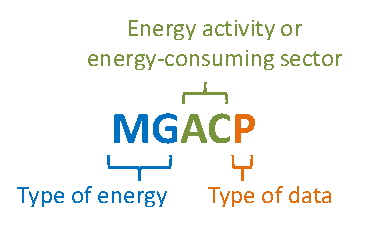
\includegraphics[width=0.3\linewidth]{fig/msn.pdf}
    \caption{Components of a MSNCODE}
    \label{fig: msn}
\end{figure}


As we can see, the first two letters of MSN code are used to represented the energy source and products, the three and four letters of MSN are used to represented the energy-consuming sectors and the last letter identifies the type of data.


Energy sources can be categorized as renewable, nuclear energy, non-renewable sources and net interstate sales of electricity:
\begin{itemize}
    \item{Non-Renewable Sources}
    \begin{itemize}
        \item {Fossil fuels}
        \begin{itemize}
            \item coal (CL)
            \item net imports of coal coke (U.S. only)
            \item natural gas excluding supplemental gaseous fuels (NN)
            \item petroleum products excluding fuel ethanol blended into motor gasoline
(PM)
            
        \end{itemize}
    \end{itemize}
    \item Nuclear electric power (NU)
    \item{Renewable Sources}
    \begin{itemize}
        \item fuel ethanol minus denaturant (EM)
        \item geothermal direct use energy and geothermal heat pumps (GE)
        \item conventional hydroelectric power (HY)
        \item solar thermal direct use energy and photovoltaic electricity net
generation (SO)
        \item electricity produced by wind (WY)
        \item wood and wood-derived fuels and biomass waste (WW)
    \end{itemize}
    \item{Net interstates sales of electricity and associated losses}
    \par
    This value can both be negative and positive, MSNCODE=ELISB.
\end{itemize}
It should be noted that due to the amount of the renewable sources are always small, we sum all the renewable sources as an energy type ’RE’. 

According to our demand and the actual situation of date provided, we select some main MSN Codes to describe the four states’ energy profiles. To check the correctness of our data, we add the total energy consumption in the data-set. Following are the details of MSN Code we used:
\begin{table}[H]
\centering
\caption{Meaning of the MSNCODE used for analyzing energy profile}
\label{tabel: msncode}
    \begin{threeparttable}
        \begin{tabular}{clc}
        \toprule
        MSN   & Description                                                           & Unit        \\
        \midrule
CLTCB & Coal total consumption.                                               & Billion Btu \\
NGTCB & Natural gas total consumption (including supplemental gaseous fuels) & Billion Btu \\
PATCB & All petroleum products total consumption                            & Billion Btu \\
NUETB & Electricity produced from nuclear power                              & Billion Btu \\
EMTCB & Fuel ethanol, excluding denaturant, total consumption               & Billion Btu \\
RETCB & Geothermal energy total consumption                                & Billion Btu \\
ELISB & Net interstate sales of electricity and associated losses (negative and positive values)                                  & Billion Btu \\
TETCB & Total energy consumption                                  & Billion Btu \\
        \bottomrule
        \end{tabular}
    \end{threeparttable}
    
\end{table}
Additional Explanation: the code of energy-consuming sectors we choose TC, but as for NU, we choose ET.

Through these steps, we finally get the energy consumption proportion and amount of the four states from 1960 to 2009, as separately shown in figure \ref{fig: prop} and figure \ref{fig: energy quantity}. In all the four states, the equation below  continuously holds:
\begin{equation}
\mathrm{TE} = \mathrm{CL}+\mathrm{NG}+\mathrm{PM}+\mathrm{NU}+\mathrm{RE}+\mathrm{EL}
\end{equation}
Note when EL is negative, which means the state exports electricity to other states, the proportion of  $\mathrm{CL}+\mathrm{NG}+\mathrm{PM}+\mathrm{NU}+\mathrm{RE}$ to the total energy will exceeds 1, and the area above 1 is the proportion of EL. When EL is positive, the blank area below 1 is the proportion of EL.
In general, the total consumption of all energy-consuming sectors increase with fluctuations, but Arizona increase fastest while New Mexico slowest. The amount of Texas and California, however, is several times that of Arizona and New Mexico. Natural gas (NG) and petroleum products (PM) is the main energy, but coal (CL) is important energy in Arizona and New Mexico still. Most of cleaner, renewable energy sources (RE) like electricity produced by wind and conventional hydroelectric power is in its infancy, but California and Arizona has a great beginning already. Specially, the Nuclear electric power (NU) has played an important role in Arizona. Besides, in the view of interstate electricity exchange, California imports more and more electricity, while Arizona and New Mexico export a relatively large proportion of electricity. Texas is nearly self-sufficient. 

\begin{figure}[H] 
    \centering 
    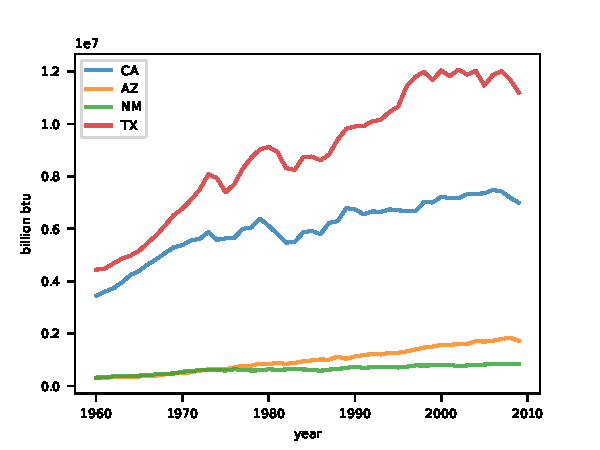
\includegraphics[width=0.5\linewidth]{fig/amount.pdf}
    \caption{Total energy consumption of the four states from 1960 to 2009}
    \label{fig: energy quantity}
\end{figure}

\begin{figure}[H] 
    \centering 
    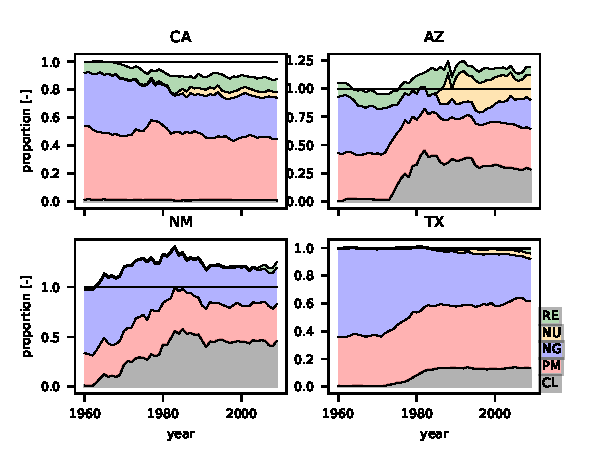
\includegraphics[width=0.8\linewidth]{fig/proportion.pdf}
    \caption{Proportion of five main energy types of the four states from 1960 to 2009}
    \label{fig: prop}
\end{figure}

\subsubsection{Summary of A}
Energy production and usage are a major portion of any economy. 
\begin{itemize}
    \item California: the energy is tending to be diverse, but the proportion of Nuclear electric power (NU) could be bigger.
    \item Arizona: the energy is tending to be diverse, and the amount increases fastest in all, but the amount is too small.
    \item New Mexico: the main energy is fossil fuels but there is little cleaner, renewable energy sources (RE).
    \item Texas: the main energy is natural gas (NG) and petroleum products (PM) and there is a little cleaner, renewable energy sources (RE).
\end{itemize}